\chapter{Introduction}
\label{chap:Introduction}



\noindent{}Honest cooperation in a population is a requirement for any level of organisation to be reliably reached. From genes, unicellular organisms, and multicellular organisms to insect colonies and human societies, the ability to cooperate is of vital importance for the survival of these species. Interactions between agents in a population can be viewed as instances of evolutionary game theory. Each interaction places two agents together whereby one agent needs the other to contribute some resource to them. Here a resource is defined in an abstract sense as any kind of helpful act that contributes to the chance for survival of a peer. This is an altruistic act of the individual, but a requirement for the survival of the entire population.\vspace{1em}\\


\section{The Evolution of Social Cooperation}
\label{sec:The Evolution of Cooperation}
\noindent{}Natural selection engenders competition among agents in a population such that selfish behaviour is rewarded. This can lead to a dilemma, commonly known as the "tragedy of the commons", in which the incentives of the individual are not aligned with those of the population as a collective. Such a dilemma is partially thwarted by the evolution of a number of mechanisms that induce cooperation in a population. Without any mechanism for the evolution of cooperation, natural selection favors defectors, which consequently outlive honest agents until there are only defectors left. Research has shown that there are 5 predominant mechanisms that biological communities adopt in order to maintain cooperation, namely {\it kin selection}, {\it direct reciprocity}, {\it indirect reciprocity}, {\it network reciprocity} and {\it group selection}. The idea behind these particular mechanisms is to reward behaviour of individuals that is beneficial to members of the population other than themselves and to some degree even punish "selfish" behaviour \cite{5 Rules for the Evolution of Cooperation}.\vspace{1em}\\


\noindent{}Agents in a population will incur some cost for performing an altruistic act, while the recipient will receive some benefit. Different mechanisms of social cooperation will yield different cost and benefit functions for altruisitc acts, based on which agents will decide whether or not it is sensible for them to cooperate. Nowak (2006) have determined under which restrictions of cost and benefit, cooperation will naturally evolve in biological communities.\vspace{1em}\\

\begin{itemize}
\item Kin Selection: Natural selection can favour cooperation if contributer and beneficiary are genetic relatives. Such an act is beneficial if the cost-to-benefit ratio exceeds the factor of relatedness, whereby the factor of relatedness is determined by the probability that both interaction partners share a gene. 
\item Direct Reciprocity: In the case of repeated encounters between the same individuals with consecutive rounds of interactions, an agent will decide whether to cooperate based on its contender's previous action. The most common form of direct reciprocity is known as the tit-for-tat strategy in game theory, which we will elaborate on later. Direct reciprocity leads to global cooperation if the cost-to-benefit ratio is exceeded by the probability of another interaction between the same agents.
\item Indirect Reciprocity: In indirect reciprocity a node cannot rely on reencountering one of its previous interaction partners, but instead is likely to encounter strangers over and over again. %resembles a barter economy, Indirect reciprocity is similar to money.
This necessitates a mechanism that works on the basis of reputation. Agents may not have the chance to reciprocate directly. Instead, people contribute to the community on the assumption that it will increase their reputation, which in turn increases the probability of them receiving some work from a stranger. This mechanism only induces cooperation if the probability of knowing someone's reputation exceeds the cost-to-benefit ratio of the interaction.
\item Network Reciprocity: We can picture this best in a graph-theoretical setting, in which every agent pays a cost for all of their neighbours in the social graph to receive a benefit. If they defect then their neighbours don't receive a benefit. Cooperators can prevail by forming network clusters among themselves, by only interacting with cooperators. This rule leads to cooperation if benefit-to-cost ratio exceeds the average number of neighbours each node has. 
\item Group Selection: The network is subdivided into groups and these groups grow as offspring is produced. As a group reaches a certain size  it splits in two and another group is eliminated. We find that defectors in a mixed group proliferate faster than honest nodes. However, groups consisting of only honest nodes split much faster than mixed groups or groups with only defectors. Hence honest groups soon dominate the network. This only happens provided that the benefit-to-cost ratio is greater than the ratio of all nodes to number of groups plus 1. \vspace{1em}\\
\end{itemize}

\noindent{}Out of all biological species there are on this planet, the human race has developed the by far most sophisticated and effective mechanism to enforce indirect reciprocity across its entire population; Language. While many other life forms on earth have developed ways of communicating with one another, humans have developed the most intricate and complex method of communication. This is the reason that from an evolutionary perspective, we have arguably outdone all other biological species on this planet. Language enables humans to {\it gossip} about one another. While this might not initially seem like a significant contributor to reproductive success, it allows humans to share information about the reliability of their peers and the likelihood that an individual will act cooperatively in the future. Based on this shared information humans can cultivate a reputation which reflects their standing in a population.  \vspace{1em}\\

\noindent{}This reputation mechanism rewards altruistic behaviour and punishes uncooperative acts. If, in an interaction with a peer an agent decides to defect then that peer will spread information about the agent's defection and if said agent has another interaction with a new peer that knows about its past defection then the agent is less likely to be collaborated with. Humans have developed an awareness of their own reputation over time which prompts them to behave cooperatively most of the time. Even with strangers whose reputation they might not know, humans often act politely and considerately, due to this awareness. While kin selection and direct reciprocity can ensure the cooperation of smaller tribes and families, reputation is a key element in the functioning of large-scale societies. \vspace{1em}\\

\noindent{}The upshot here is that bad behaviour is punished with bad reputation, while good behaviour is rewarded with good reputation. Good reputation leads to trust between two individuals, which results in more effective cooperation between individuals. Lastly, humans have incorporated "forgiveness" into this scheme. Individuals' reputations are malleable and dynamic. Agents that have misbehaved and developed a bad reputation can change their behaviour and redeem themselves, correcting their wrong-doings and fixing their reputation. This upgrades the reputation mechanism and ensures that defectors are incentivised to rectify their strategy and become cooperators.\vspace{1em}\\


\section{Cooperation and Behaviour on the Internet}
\label{sec:Cooperation and Behaviour on the Internet}
\noindent{}With the advent of one of the most disruptive technological revolutions in human history, namely the Internet, humans have been given an entirely new platform to interact on globally. There are a wide variety of different networks in which different types of resources are shared, from P2P file sharing networks, where agents up- and download data to one another to social networks where humans interact by sharing content with one another and rewarding or chastising it with "likes" or "retweets", etc. The social graph of human interaction has changed and especially grown significantly with the help of these tools. This changes the paradigm of human interaction and consequently their behaviour. It has been commonly observed that people are often much "nastier" to one another on the Internet than they are in real life. This nastiness can be considered as a form of defection against paradigms of social interaction, leading us to believe that the aforementioned rules for inducing cooperation no longer function effectively.\vspace{1em}\\

\noindent{}On the Internet humans no longer interact face-to-face and, more importantly, no longer need to disclose their identity to one another. Identity, however is an indispensable input of any reputation mechanism. For a reputation mechanism to be effective, identities need to be permanent and unique. When humans have the ability to hide their identity behind one or several pseudonyms, they can defect without having to face any long-term repercussions. Malicious peers may hide behind one or several pseudo-identities or even erase previous identities entirely in order to avoid bad reputation as a result of bad behaviour. The regular mechanisms for cooperation are no longer applicable and a new online analogue to reputation might have to be devised. This problem becomes particularly apparent in online social networks.\vspace{1em}\\

\noindent{}Social networks such as Facebook and Twitter, etc. struggle to clamp down on malicious behaviour such as cyberbullying and the proliferation of hateful content or "fake news". In the physical world this type of behaviour would be strongly disincentivised by the mechanisms of cooperation given in \ref{sec:The Evolution of Cooperation}. A bully for instance, will be socially frowned upon and become an outcast from the community if their behaviour is not rectified. Of course, even in the real world these cooperative mechanisms are not implemented perfectly, however they do work. On the Internet, due to the reasons discussed above, we find that this is no longer the case. Reputation is no longer a reliable piece of information and trust is harder to achieve, making these networks increasingly uncooperative environments. While companies running these networks do their best in utilising technology to prevent and mitigate bad behaviour, they have so far not succeeded entirely.\vspace{1em}\\ 


\section{Cooperation in Peer-to-peer Filesharing Networks}
\label{sec:Cooperation in Peer-to-peer Filesharing Networks}
\noindent{}Another preeminent setting in which this problem of cooperation arises are online P2P filesharing networks. Peer-to-peer file sharing refers to the distribution of digital media over a P2P network without the need for any central authority or database. Files are located on individuals' computers and shared with other members of the network through up- and downloading data to one another. P2P software was the piracy method of choice in the early 2000s with software programmes such as LimeWire, Gnutella and the BitTorrent client being the most prominent applications \cite{The Early Days of Mass Internet Piracy Were Awesome Yet Awful}. A Supreme Court decision in 2005 led to the closure of many of these sites for illegally sharing copyrighted material. However, these applications are still very much in use today.\vspace{1em}\\

\noindent{}In P2P file sharing networks agents up- and download files amongst one another through acts called {\it seeding} and {\it leeching}. Agents holding a particular file will receive requests for the given file they are holding by so-called leechers. Nodes that require a particular file join a swarm of other nodes with the same needed file. Agents willing to seed now have to decide who to make a contribution to. The file they are willing to share is split into smaller pieces which are distributed among members of the swarm in a manner that ensures a fair distribution and prevents data from going extinct when agents go offline or leave the mesh. \vspace{1em}\\

\noindent{}P2P filesharing networks are an instance of computing distributed systems, which do not have any central authority governing the network. Instead of connecting to a central server for data, agents interact freely in a decentralised manner as visualised in figure \ref{fig:Client-Server vs P2P Model}. \vspace{1em}\\


\begin{figure}[H]
\begin{center}
\includegraphics[scale=0.75]{"Central vs Decentralised".PNG}
\caption{Client-Server vs P2P Model}
\label{fig:Client-Server vs P2P Model}
\end{center}
\end{figure}

\noindent{}There are some advantages and some disadvantages of the distributed nature of P2P networks over the traditional client-server model and their applicability depends on the context. The most notable are listed in the table given in figure 1.2 below.\vspace{1em}\\

\begin{figure}[H]
\begin{center}
\begin{tabular}{|c|c|}
\hline & \\[-0.7ex] \textbf{Advantages:} & \textbf{Disadvantages:} \\[1.5ex] \hline & \\[0.7ex]
No single point of failure & No Accountability \\
No network congestion & Possible malware on the network \\
No expensive server architecture needed  & No backup of data \\
 & Updates are difficult to implement \\[1ex] 
\hline
\end{tabular}
\label{fig:Pros and Cons of P2P}
\caption{Advantages and disadvantages of P2P over Client-Server}
\end{center}
\end{figure}

\noindent{}In most online networks with some kind of central authority, such as Ebay, Airbnb, etc. cooperativeness is achieved through review mechanisms, which are maintained and secured by the central authority. Agents can evaluate the trustworthiness of their potential interaction partners, by assessing their previous transactions and other agents' opinions of them. These reviews are stored on a central database which the central authority maintains. Seeing as the point behind P2P networks was to eliminate this central authority the problem of cooperation arises again. Users have an obvious incentive to download, but no inherent incentive to share data. This is what we referred to earlier as {\it the tragedy of the commons}, which results in behaviour we call {\it lazy freeriding}, where agents leech excessively, but do not seed. Different file sharing platforms have different mechanisms to enforce the necessary altruistic sharing of files. \vspace{1em}\\


\subsection{BitTorrent \& Direct Reciprocity}
\label{subsec:BitTorrent & Direct Reciprocity}
\noindent{}To facilitate cooperation the most prominent P2P network, BitTorrent, employs a mechanism called {\it tit-for-tat}, which is an instance of direct reciprocity. Tit-for-tat is a highly effective strategy in game theory for the iterated prisoner's dilemma, in which an agent cooperates first and then replicates its contender's previous actions as seen in figure \ref{fig:Instance of the Prisoner's Dilemma, in which Tit-For-Tat is the Dominant Strategy}. In practice, this works as follows. Peers in the BitTorrent network have a limited number of upload slots to allocate. An agent will begin by exchanging upload bandwidth for download bandwidth with a number of its peers. If one of these peers turns out to be a leecher, i.e. does not reciprocate, it will be choked out. This means the agent will discontinue it's cooperation and assign the corresponding upload slot to another randomly chosen peer in a procedure known as {\it optimistic unchoking}. \vspace{1em}\\

\begin{figure}[H]
\begin{center}
\includegraphics[scale=0.7]{"Tit-4-Tat".jpg}
\caption{Instance of the Prisoner's Dilemma, in which Tit-For-Tat is the Dominant Strategy. Image taken from \cite{Prisoner's Dilemma Image}.}
\label{fig:Instance of the Prisoner's Dilemma, in which Tit-For-Tat is the Dominant Strategy}
\end{center}
\end{figure}

\noindent{}However, we find that in the case of fleeting and asymmetric interactions, tit-for-tat is no longer very effective \cite{A Simple Rule for the Evolution of Cooperation on Graphs and Social Networks}. Fleeting and asymmetric means that agents have many unrepeated and unreciprocable interactions with their peers. When there is a high probability of two agents not seeing each other again, peers cannot be evaluated based on their previous reliability and hence every new transaction entails the risk of the contender defecting. In tit-for-tat agents do not keep a memory about their peers' reliability and do not share information about this behaviour with the network. In such a setting defecting becomes the dominant strategy of the Prisoner's dilemma \cite{An Optimal Strategy to Solve the Prisoner's Dilemma}. The agents' inability to coordinate and build expectations of their counterparts ensures that defection will rarely be punished. Everyone is worse off than if they had collaborated, but no individual can gain anything by changing to a collaborative strategy, since there's almost never a reward. This is what we referred to as the tragedy of the commons earlier in section \ref{sec:The Evolution of Cooperation}. We find that a mechanism of indirect reciprocity may be more successful at inducing cooperation in these types of networks. \vspace{1em}\\


\subsection{Tribler \& Indirect Reciprocity}
\label{subsec:Tribler & Indirect Reciprocity}
\noindent{}The {\it Distributed Systems Group} at Delft University is running and developing an open-source P2P file sharing network, called {\it Tribler}, which aims to leverage the power of mechanisms for social cooperation in an attempt to create a more reliable file sharing platform. It is designed with a custom built-in onion routing network whereby the transference of data is routed through several relay nodes before reaching the leeching node, ensuring anonymity of participants and clients can participate in any BitTorrent network. Tribler is trackerless and built on an overlay network for content searching, rendering it truly decentralised and immune to limiting external action such as government restraint.  \vspace{1em}\\ 

\noindent{} \begin{center}Johan Pouwelse. „The only way to take down Tribler is to take down the Internet.“ (Dailymail 2009) \vspace{1em}\\\end{center}

\noindent{}In an attempt to alleviate the problem of freeriding, Tribler aims to incorporate mechanisms of {\it indirect reciprocity} to enforce cooperation. Agents gossip about their transaction partners and inform others about their trustworthiness. Agents' respective transaction histories are disseminated along the network. From this information agents can aggregate an approximation of their peers' reputations such that freeriders and otherwise uncooperative agents can be identified. An agent that holds parts of a particular file will receive queries from peers that require that particular file just like in the BitTorrent protocol. The agent holding the file will then decide whom to upload to, based on the reputation of the nodes in the swarm. After having some work performed the reputation of the performer should increase while that of the recipient should decrease, such that in the next interaction the peer that has performed the work will have a higher probability of receiving work and the recipient will have a lower one. Uncooperative nodes are therefore not completely shunned, but are restrained in their ability to consume data. \vspace{1em}\\

\section{Blockchains and TrustChain to Enhance Online Cooperation}
\label{sec:Blockchains & TrustChain}
\noindent{}In order for agents to be able to evaluate their peers' reputation based on their respective transaction histories there needs to be a database logging all agents' interaction histories. However, seeing as it's Tribler's goal to avoid any kind of centralisation, a distributed storage, or ledger, is required. The most commonly used tool for this purpose are Blockchains. Blockchains are append-only data structures that utilise cryptographic primitives such as public-key cryptography and digital signatures to maintain a consensus on data, stored on many different processors in a distributed system. Transactions between agents in the network are grouped in blocks which, in turn, are interlinked by a hash chain. \vspace{1em}\\

\noindent{}The most popular type of blockchain is given by the Bitcoin proof-of-work blockchain, in which blocks are created by "miners"; nodes in the network that collect and group transactions. In order to obtain a block, the miner needs to solve a crpytographic hash puzzle through a protocol known as proof-of-work (PoW). If conflicting states occur, the chain forks, and miners contribute to the chain they believe is the valid one. At some point, one chain will overtake the other and all miners transition to {\it that} chain. This point is determined by a certain number of blocks by which one chain surpasses the other, which is based on a predetermined lower bound for the probability of a dishonest miner single-handedly overruling the current chain. The resulting chain of blocks is therefore immutable as well as fraud-proof. The idea behind behind PoW and miners is that authority to make changes to the log is randomised, making it impossible for any single agent to obtain any significant authority over what is stored on the Blockchain \cite{Bitcoin}. \vspace{1em}\\

\noindent{}Blockchains however have a major drawback that the classical client-server model does not have. In order to ensure randomisation of append-authority and transaction validity agents are required to wait for a certain number of blocks to exceed a transaction's block before this transaction is deemed valid. This fundamentally limits their scalability in terms of transaction throughput. In pursuing a more scalable alternative, the distributed systems group of the TU Delft has developed their own type of distributed ledger, called TrustChain \cite{TrustChain: A Sybil-resistant scalable blockchain}. TrustChain is what is known as a fourth-generation blockchain. \vspace{1em}\\

\noindent{}Unlike most traditional blockchains, all network participants maintain their own chain of transactions in the TrustChain protocol. There is no mining and no global consensus. The TrustChain maintains records of all interactions between peers in the network, in respective blocks. Blocks are linked to one another through hash pointers, whereby a block contains the hash value of its preceding block. Each block is thereby connected to two preceding and two succeeding blocks, i.e. each block is contained in the chains of both transaction partners. This results in many interlinked chains, each corresponding to a single agent's transaction history. For a visualisation of the TrustChain datastructure see Figure \ref{fig:Trustchain}. \vspace{1em}\\

\begin{figure}[H]
\begin{center}
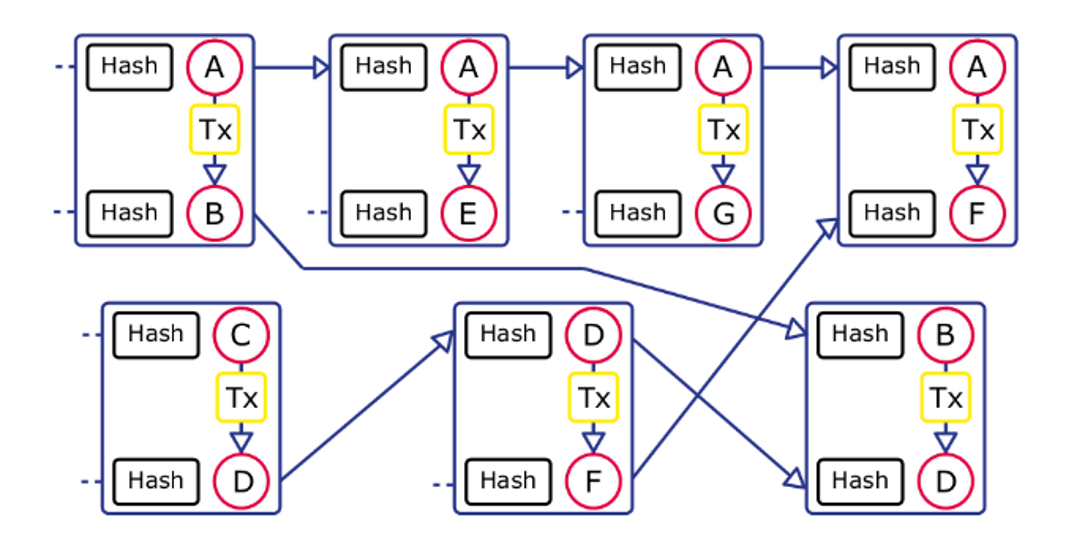
\includegraphics[scale=0.5]{Trustchain.png}
\caption{TrustChains of different network participants (taken from \cite{TrustChain: A Sybil-resistant scalable blockchain}).}
\label{fig:Trustchain}
\end{center}
\end{figure} 

\noindent{}This structure is strongly scalable, both in the number of agents in the network as well as in the number of transactions per agent as TrustChain does not maintain a global consensus. This means that double-spend attacks are not actually prevented, as they are in traditional blockchains. However, they are made detectable through a gossip-protocol, as peers share information about other nodes' transaction histories and can subsequently be penalised. Thereby fraudulent activity is not actually prevented, but strongly disincentivised.\vspace{1em}\\


\newpage
\chapter{Research Question}
\label{chap:Research Question}
\noindent{}The Tribler P2P network aims to incorporate a reputation mechanism into their application to enforce indirect reciprocity and thereby achieve cooperation. Ultimately, the goal is to determine an algorithm that takes the TrustChains of agents participating in the network and returns some reputation scores for these nodes. Reputation is subjective and therefore reputations should be determined by all nodes independently based on the data they have gathered through the gossip protocol. There are many algorithms that spring to mind that may achieve a desirable outcome in this setting. However, designing such an algorithm comes with a particular set of challenges that must be overcome for it to be effective. This leads us to our research question:

\begin{center}
\noindent{}{\it What requirements does a reputation mechanism need to satisfy to induce cooperative behaviour in a P2P file sharing network?} \vspace{1em}\\
\end{center}
 
\noindent{}In order to answer this question we begin by refining our understanding of a reputation mechanism. In \cite{On the Sybil-Proofness of Accounting Mechanisms} Seuken \& Parkes (2011) introduce the concept of {\it accounting mechanisms} which are mappings on a social interaction graph representing the reputability that agents in the P2P network have based on their interaction histories. If one agent is assigned a higher score than another agent by this mapping then that agent is considered more reputable. The main idea is that a sensible accounting mechanism should assign higher scores to nodes who make overall larger contributions to the network and consume less than other nodes. A node with a higher reputation score should then find itself more likely to be served data, therefore stimulating cooperative behaviour. Conversely, agents that behave selfishly should be assigned lower reputation scores and should therefore be less likely to receive data, disincentivising selfish behaviour. \vspace{1em}\\

\noindent{}Ideally, accounting mechanisms should entail some transitivity, by which we mean nodes assign agents that they have had direct interactions with higher reputation scores than nodes they have not had direct interactions with. The larger the distance between two nodes in the social interaction graph the smaller the reputational reward for a contribution. Additionally, contributions that are indirect contributions to a node should lead to higher reputation scores than contributions that are not indirectly benefitting this node. By indirect contributions we mean that if a node contributes some resources to another node which in turn serves a third node, then the third node will consider the contributions made by the first node indirect contributions to itself. This would accurately capture the concept of reputation as encountered in the real world. \vspace{1em}\\ 

\noindent{}Lastly, an accounting mechanism should successfully prevent \textbf{lazy freeriding}. We consider an agent that consumes far more resources than they contribute a lazy freerider. More rigorously, we say that if the net contributions a node has made to the rest of the network, i.e. the amount they have consumed subtracted from the amount they have contributed, exceed a certain lower bound then that node is a lazy freerider. Alternatively, we might say that if the ratio of these values exceeds a given lower bound then that node is a lazy freerider. An accounting mechanism should penalise excessive leeching in a manner that makes it impossible for a node to go below such a threshold.\vspace{1em}\\

\noindent{}So far, this question seems like a rather easy one to solve. There are plenty of algorithms that will capture these requirements and prevent lazy freeriding. However, the question is complicated by the possibility of attacks on the file sharing network. In this work we will focus on two types of attacks in particular, namely misreport attacks and sybil attacks. \vspace{1em}\\


\noindent{}A {\bf misreport attack} is performed by one or more malicious agents who do not report honestly on their own past interactions. Malicious agents may try to deceive honest agents by reporting on transactions that have not actually occurred or by concealing transactions  that may reduce their standing in the network. By this method agents can increase their reputation or reduce the standing of other nodes in the network. In \cite{Accounting Mechanisms for Distributed Work Systems} Seuken \& Parkes (2011) have introduced a mechanism which solves this problem to some degree. In this work we examine the ability of the TrustChain architecture to prevent this type of attack. \vspace{1em}\\ 

\noindent{}A {\bf sybil attack} occurs when a single malicious agent creates multiple, often times large amounts of, fake identities. This agent will then attempt to exploit the control they have over the accounts in order to artificially increase the reputation score of one or more of their identities by reporting high levels of reputability through fake transactions without actually performing any work. Another approach may be to simply reduce the reputation of other honest nodes in the network to improve their own relative standing(s). This can be done because Sybil identities can create forged reports about one another. Such attacks can have strongly detrimental effects on the functioning of P2P networks, especially if carried out on a large scale. If the creation of identities and forging of transactions are cheap compared to their gain, then such attacks have the potential to disrupt entire file-sharing networks.  \vspace{1em}\\

\noindent{}Given these types of attacks we can narrow down our research question to the following
\begin{center}
{\it What requirements does an accounting mechanism need to satisfy in order to effectively incentivise cooperation and prevent lazy freeriding, while being resistant to misreport attacks and mitigating the effects of sybil attacks?}
\end{center}

\begin{comment}
\subsection{Other Types of Attacks}
\label{subsec:Other Types of Attacks}
\noindent{}There are many other types of attacks one can perform to disrupt p2p networks and we will not be able to analyse the effects of all of these in this thesis. Some of the more prominent attacks are mentioned below. Note however, that the main focus of our thesis will, from here on out, lie on preventing lazy freeriding and mitigating sybil attacks. \vspace{1em}\\

\subsubsection{Collusion Attacks}
\label{subsubsec:Collusion Attacks}
\noindent{}Collusion attacks resemble sybil attacks in that a group of nodes cooperate in an attempt to behave maliciously without being punished or detected. The difference between these types of attacks and sybil attacks lies in the fact that the colluding agents are controlled by different parties and may be far away from each other, geographically. In a sybil attack the nodes that collude are controlled by one and the same party. An example of a collusion attack my be given by several nodes getting together and reporting positive transactions about one of their members $j$ to an honest node $i$. This increases the chances of $j$ being served some data by $i$, which it may then, in turn, distribute to other participants of the collusion attack. This type of attack is very difficult to prevent as there may not be any noticeable sign of it in the work graph. Luckily these types of attack are quite rare and usually not that beneficial as there is an inherent problem of trust among the malicious nodes.\vspace{1em}\\

\subsubsection{Eclipse Attacks}
\label{subsubsec:Eclipse Attacks}
\noindent{}An eclipse attack lies halfway between a sybil attack and a misreport attack. A malicous agent $j$ may choose to impersonate multiple identities in the network in an attempt to shield an innocent node from the rest of the network. The goal is to prevent the attacked node from obtaining reports about certain transactions in the network and therefore to isolate it in a part of the network that is predominantly malicious and controlled by the attacker. \vspace{1em}\\

\subsubsection{Malware Distribution \& and DDoS Attacks}
\label{subsubsec:Malware Distribution & and DDoS Attacks}
\noindent{}Another way of attacking the network is by injecting useless data and/or even malware into the network, thereby "poisoning" the traffic. The intent may either be to directly attack individual peers by providing them with camouflaged corrupted files, or to simply choke of network traffic. This can be done by inserting fake records into the index pointing to a target IP and port number. When an agent then looks up a file it will receive fake location information from a poisoned index. This can slow the network traffic to a crawl. \vspace{1em}\\

\subsubsection{Whitewashing Attacks}
\label{subsubsec:Whitewashing Attacks}
\noindent{}Lastly, a whitewashing attack occurs when an agent deletes their identity from the network and starts from scratch with a new identity. This way an agent can whitewash their history in the network. This is done to evade negative repercussions of malicious behaviour and start afresh as a newcomer node. An example for this may be an agent in a social media network that has been exposed as distributing malignant content, closing and reopening a new account, only to resume the same strategy.\vspace{1em}\\  
\end{comment}


\begin{comment}
\section{Related Work}
\label{sec:Related Work}
\noindent{}The body of literature researching reputation mechanisms on social interaction graphs is quite large and we have limited our scope, for the most part, to the research conducted by authors Seuken and Parkes, who have made large contributions to the research of this exact question. The research that we focused on the most throughout this thesis is their paper titled "On the Sybil-Proofness of Accounting Mechanisms", in which they discuss some impossibility results for the prevention of sybil attacks \cite{On the Sybil-Proofness of Accounting Mechanisms}. They define 3 requirements accounting mechanisms must satisfy in order for them \textbf{not} to be sybil resistant. Later they relax their definition of sybil-proofness to only include up to $K$ sybil identities and introduce two additional restrictions for accounting mechanisms to satisfy this definition of sybil resistance. We will critically examine these results and expand on their research. \vspace{1em}\\

\noindent{}The same authors have produced a variety of results to ensure the resistance of accounting mechanisms against misreport attacks and sybil attacks. Their most notable mechanism against misreports is called DropEdge defined in \cite{Accounting Mechanisms for Distributed Work Systems} and expanded in \cite{Sybil-proof Accounting Mechanisms with Transitive Trust}, which we will reintroduce in this thesis and compare to Tribler's TrustChain architecture \cite{TrustChain: A Sybil-resistant scalable blockchain}. \vspace{1em}\\

\noindent{}They have also evaluated a number of different graph theoretical centrality measures in their applicability in this problem, such as the PageRank algorithm, a maximum-flow based centrality measure called BarterCast as well as a hitting time algorithm. They analysed their resistance to sybil attacks by various metrics such as rank-strategyproofness, value-strategyproofness and upwards value-proofness as well as relaxed versions of these metrics \cite{Hybrid Transitive Trust Mechanisms}. Other metrics for the evaluation of accounting mechanisms are informativeness, misreport-proofness and long-term misreport-proofness \cite{Sybil-resistant Trust Mechanisms in Distributed Systems}. \vspace{1em}\\ 

\noindent{}They discuss some more properties of accounting mechanisms, such as work-monotonic transitive trust and strong transitive trust, narrowing down the definition. Lastly, they invent the concept of hybrid transitive trust mechanisms, which are the convex combination of accounting mechanisms. These may satisfy nice properties than "single" accounting mechanisms as they may combine nice properties of several accounting mechanisms \cite{Hybrid Transitive Trust Mechanisms}.\vspace{1em}\\

\noindent{}Another very relevant piece of work is Otte's "Sybil-resistant trust mechanisms in distributed systems", in which a completely new accounting mechanism, called netflow, is introduced. The authors evaluate this mechanism based on the metrics given above. The authors show that this mechanism satisfies sybil-resistant according to the definition given by the authors above. Lastly, they also examine the temporal pagerank algorithm as a possible accounting mechanism and its resistance to sybil attacks under a given time restriction.\vspace{1em}\\  
\end{comment}

\begin{comment}
\item[Sybil-proof Accounting Mechanisms with Transitive Trust:] They introduce the concept of strong transitive trust (think through and explain nicely later). They also introduce the concept of long-term misreport-proofness, which include dynamic graphs (i think...). They claim that dropedge is long-term misreport-proof. They refine the concept of weakly beneficial sybil attacks, but still keep the ambiguity in it. They state a new impossibility theorem. Then introduce weak transitive trust and a new variant of drop-edge and claim that the two will still yield weakly beneficial sybil attacks. They then show that their theorem is "tight", which means that if any of the things dicussed above are not satisfied anymore the assertion no longer holds.
\item[Hybrid Transitive Trust Mechanisms:] They work on the trust graph and introduce the definition of transitive trust mechanisms (here they rewrite their accounting mechanism the way we did). Here they finally define misreport!!! Quite similar to us, except they have culprite while we don't. They introduce rank-strategyproofness and value-strategyproofness. Examples of transitive trust mechanisms PGR, Hitting Time, MaxFlow, ShortesPaths then they explain whether these are rank-and value-strategyproof. They come up with hybrid mechanisms, where you take two mechanisms and take convex combo of them. Then they have theorems about value-and rank-strategyproofness of hybrid mechanisms. They relax their notions of these things to eps-rank(values) strategyproof and make statements of about hybrid mechanism strategyproofness. They have some examples of which mechanisms satisfy this. They relax value-strategyproofness to upwards value-proofness and extend their results. 
\item[Otte:] Introduce interaction model, which we will disagree with as it doesn't have possibility for misreports. Very nice for TrustChain though. Make the same mistake with sybil attack profit. Come up with their own accounting mechanism called Netflow limited contribution. Then they show that it is resistant to weakly beneficial sybil attacks. They introduce definition of informativeness.. it's not so informative, so they scale it to be more informative. They discuss some weaknesses of netflow and its resistance to other attacks. They then discuss temporal pagerank and simulate it... 
\end{comment}


\section{Thesis Summary and Contributions}
\label{sec:Thesis Summary and Contributions}
\noindent{}In chapter \ref{chap:Mathematical Framework for Accounting Mechanisms} we begin by mathematising the relevant concepts such as transactions, work graphs, accounting mechanisms, allocation policies, lazy freeriding, misreports, sybil attacks and the TrustChain architecture. We prove the resistance of accounting mechanisms that are based on the TrustChain architecture to misreports under some mild restrictions and we prove the resistance of certain types of accounting mechanisms to lazy freeriding. This chapter is meant to simply provide a framework in which we can conduct our research. \vspace{1em}\\

\noindent{}In chapter \ref{chap:Sybil Attack Gain} we elaborate on the effects of sybil attacks. We introduce the concept of its cost and profit for the attacker. The cost of a sybil attack turns out to be easily explained, while defining the profit turns out to be more involved. We solve this problem by postulating an interaction model in which we also evaluate which allocation policies are most resistant to sybil attacks. Given this model we can determine a formula for the profit of a sybil attack. This is the amount of additional work that can be consumed by the attacker after the attack has been carried out. Seeing as this formula is based on a discrete stochastic process we realise that it is impossible to compute in a generic setting. In order to obtain values for the cost and profit of a sybil attack that are practically computable we redefine these values for accounting values, i.e. the aggregate of additional accounting values obtained by the attacker and its sybils. We believe that rigorous definitions of these terms are much needed and have been neglected in the existing literature such as in \cite{On the Sybil-Proofness of Accounting Mechanisms}. \vspace{1em}\\

\noindent{}The values of sybil attack cost and profit in terms of accounting values are now much easier to compute. However, they are not actually the relevant metric, but just a proxy for the earlier defined cost and profit of sybil attacks in terms of work. Given these two different definitions we investigate the relationship between them. We introduce examples where the two above are not equivalent in chapter \ref{chap:Representativeness of Accounting Mechanisms}. This turns out to be very problematic indeed as accounting mechanisms only serve as a representation of a node's cooperativeness and a sybil attacker aims to increase these in an attempt to obtain more work from the network. Therefore we find that some accounting mechanisms do not allow for accurate assessment of sybil attack profit. In order to circumvent this dilemma we come up with the definition of representativeness to ensure consistency between these two concepts of sybil attack profit.\vspace{1em}\\

\noindent{}In chapter \ref{chap:On the Impossibility of Sybil-Proofness} we analyse existing impossibility results from the literature which state under which conditions accounting mechanisms are susceptible to sybil attacks that enable the attackers to consume large amounts of data \cite{On the Sybil-Proofness of Accounting Mechanisms}. We detect an error in an important theorem and extend the existing model to circumvent this error. We introduce two additional properties of accounting mechanisms which ensure the existence of impactful sybil attacks and produce two further impossibility results as well as consequent corollaries for slightly relaxed versions of the two properties.\vspace{1em}\\

\noindent{}In our last chapter, chapter \ref{chap:Sybil-Proofness of Accounting Mechanisms} we aim to do the inverse of what we did in chapter \ref{chap:On the Impossibility of Sybil-Proofness}, i.e. introduce properties for accounting mechanisms to be resistant to strongly beneficial sybil attacks. We begin by characterising certain types of passive sybil attacks, namely parallel and serial attacks. Next, we introduce requirements for accounting mechanisms to be resistant to these types of attacks. We extend the model to a particular type of sybil attack to which accounting mechanisms that are resistant to the upper types of attacks, are also resistant. Lastly, we extend our requirements for accounting mechanisms by an aditional property to be obtain resistance to arbitrary types of sybil attacks as well. \vspace{1em}\\

\noindent{}In the appendix in chapter \ref{chap:Appendix} we address research we conducted that did not turn out to be fruitful. The first approach to solving this problem was through a model based on geographic proximity of participants in the network. The second topic we analysed was the topic of the evolution of cooperation among biological organisms. For this we made a month long research visit to Japan to analyse properties reputation mechanisms should satisfy to be able to facilitate cooperative behaviour. \vspace{1em}\\

\begin{comment}
\begin{itemize}
\item We critically evaluate existing literature, especially Seuken \& Parkes impossibility results (found mistakes)
\item We introduce much needed definition of sybil attack cost profit (lead to error in impossibility results)
\item We introduce additional constraints for accounting mechanism impossibility results
\item We introduce definition of representativeness to fix incongruence of attack cost and profit
\item We characterise sybil attacks and introduce requirements for accounting mechanisms to be sybil resistant
\end{itemize}
\end{comment}